\documentclass[border=3pt]{standalone}
\usepackage{tikz}
\usepackage{tikz-3dplot}
\usetikzlibrary{shapes,calc,positioning}

\definecolor{neworange}{RGB}{211,51,0}
\definecolor{salmon}{RGB}{255, 127, 80}
\definecolor{yellowstone}{RGB}{ 245, 176, 65 }
\definecolor{graphite}{RGB}{46, 64, 83}

\begin{document}

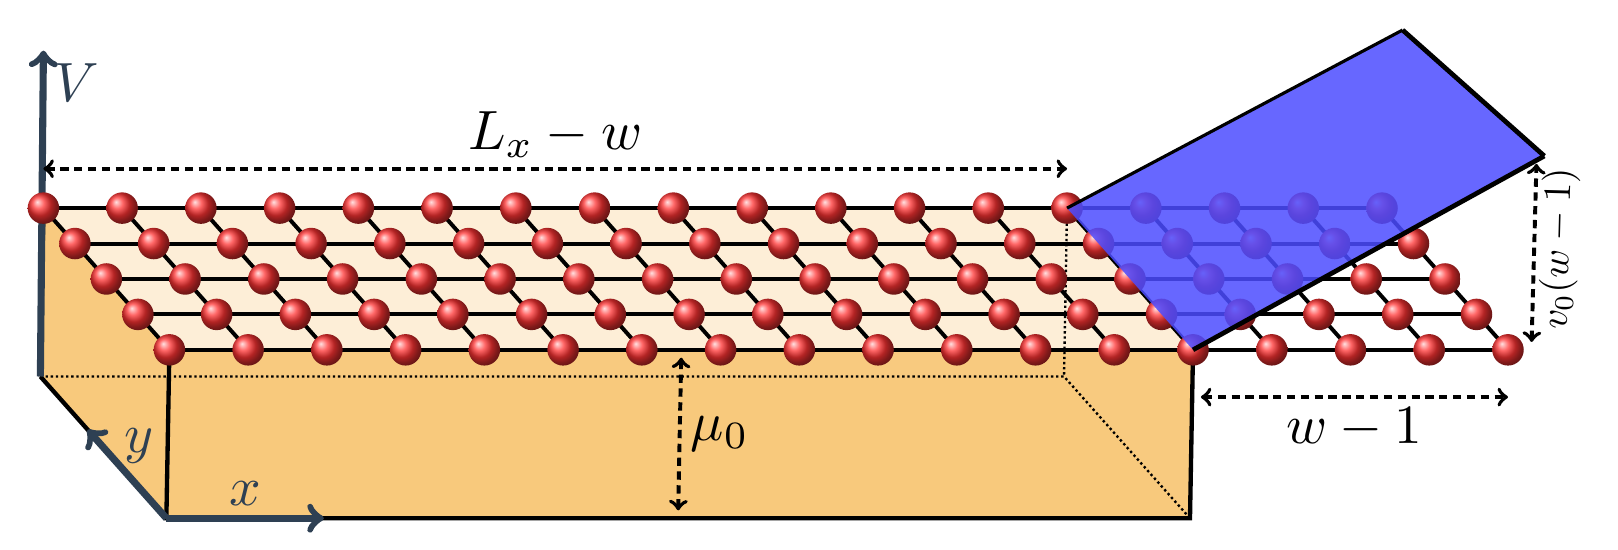
\begin{tikzpicture}[axis/.style={->,dashed},thick]

% Lattice dimensions (Lx,Ly)
\def\Lx{17} % Cells along-x
\def\Ly{4}  % Cells along-y
\def\Jump{-0.4}
\def\xwidth{1.0}
\def\ywidth{0.45}
\def\confwidth{4}


\coordinate  (d01) at (0,0,0){};
\coordinate  (d02) at (\Jump*\Ly , \ywidth*\Ly, 0){};

\coordinate  (d1) at (0,3,0.5){};
\coordinate  (d2) at (\Jump*\Ly,\ywidth*\Ly + 3,0.5){};

\coordinate  (d03) at (\confwidth + \Jump*\Ly,\ywidth*\Ly,0){};
\coordinate  (d04) at (\confwidth,0,0){};


\coordinate  (d03p) at (\Jump*\Ly,\ywidth*\Ly,0){};
\coordinate  (d04p) at (0,0,0){};
\coordinate  (d3p) at (\Jump*\Ly,\ywidth*\Ly - 2.1,0.1){};
\coordinate  (d4p) at (0,-2.1,0.1){};


\coordinate  (d3) at (\confwidth + \Jump*\Ly,\ywidth*\Ly + 2.1,0.1){};
\coordinate  (d4) at (\confwidth,2.1,0.1){};


%%%%%%%%%%%%%%%Left Wedge
%\fill[fill=blue!70, opacity=0.75] (d01) -- (d1) -- (d2) -- (d02) -- cycle;
%\fill[fill=blue!70, opacity=0.5] (d1) -- (d2) -- (d03) -- (d04) -- cycle;
%\fill[fill=blue!70, opacity=0.75] (d01) -- (d1) -- (d04) -- cycle;

%\draw[line width=0.5 mm, black, densely dotted] (d01) -- (d1) -- (d04);
%\draw[line width=0.5 mm, black, densely dotted] (d02) -- (d2) -- (d03);
%\draw[line width=0.5 mm, black, densely dotted] (d1) -- (d2) node[midway,left] {\scalebox{1.5}{$V_o$}};


%%%%%%%%%%%%%%%Rectangle
\coordinate  (d06) at (\Lx-\confwidth + \Jump*\Ly,\ywidth*\Ly,0){};
\coordinate  (d05) at (\Lx-\confwidth,0,0){};

\coordinate  (d6) at (\Lx-\confwidth + \Jump*\Ly,\ywidth*\Ly -2.1,0.1){};
\coordinate  (d5) at (\Lx-\confwidth,-2.1,0.1){};

\fill[fill=yellowstone!70, opacity=0.95] (d03p) -- (d3p) -- (d4p) -- (d04p) -- cycle;
\fill[fill=yellowstone!70, opacity=0.95] (d04p) -- (d4p) -- (d5) -- (d05) -- cycle;
\fill[fill=yellowstone!70, opacity=0.3] (d05) -- (d5) -- (d6) -- (d06) -- cycle;
\fill[fill=yellowstone!70, opacity=0.75] (d3p) -- (d4p) -- (d5) -- (d6) -- cycle;
\fill[fill=yellowstone!70, opacity=0.3] (d03p) -- (d3p) -- (d6) -- (d06) -- cycle;

\draw[line width=0.55 mm, black] (d04p) -- (d4p) -- (d5) -- (d05);
\draw[line width=0.3 mm, black, densely dotted] (d3p) -- (d6) --(d5);
\draw[line width=0.55 mm, black] (d03p) -- (d3p);
\draw[line width=0.3 mm, black, densely dotted] (d06) -- (d6);
\draw[line width=0.55 mm, black] (d4p) -- (d3p);

\draw[->,line width=0.9mm,graphite] (\Jump*\Ly, \ywidth*\Ly -2.1, 0.1) -- (\Jump*\Ly, \ywidth*\Ly+2, 0.0) node [right=12pt,below] {\scalebox{2}{$V$}};

%Lattice connections:
\foreach \x in {0,...,\Lx} {
    \foreach \y in {0,...,\Ly} {
        % Apply isometric projection for start points
        \pgfmathsetmacro{\xpos}{\x +\Jump*\y}
        \pgfmathsetmacro{\ypos}{\ywidth*\y}
        
        % Connect horizontally (x direction)
        \ifnum\x<\Lx
            \pgfmathsetmacro{\xnext}{\x + \xwidth + \Jump*\y}
            \pgfmathsetmacro{\ynext}{\ywidth*\y}
            \draw[line width=0.5 mm, black] (\xpos, \ypos) -- (\xnext, \ynext);
        \fi
        % Connect vertically (y direction)
        \ifnum\y<\Ly
            \pgfmathsetmacro{\xnext}{\x + \Jump*(\y+1)}
            \pgfmathsetmacro{\ynext}{\ywidth*(\y+1)}
            \draw[line width=0.5 mm, black] (\xpos, \ypos) -- (\xnext, \ynext);
        \fi
    }
}


% Loop to create the 3D lattice
\foreach \x in {0,...,\Lx} {
    \foreach \y in {0,...,\Ly} {
        
        %Isometric projection for 3D effect
        \pgfmathsetmacro{\xpos}{\x + \Jump*\y}
        \pgfmathsetmacro{\ypos}{\ywidth*\y}
        
        % Draw each lattice point
%        \fill[black] (\xpos, \ypos) circle (0.1);
%        \filldraw[fill=red, draw=red](\xpos-0.05,\ypos-0.05) circle (0.05);
% 		 \draw[fill=red, rotate around={-45:(1.0*\xpos,1.0*\ypos)},magenta] (1.0*\xpos,1.0*\ypos) ellipse (0.1 and 0.14);
		 \shade[ball color=red!80] (\xpos, \ypos) circle (0.2);
    }
}


%%%%%%%%%%%%%%%Right Wedge
\coordinate  (d07) at (\Lx + \Jump*\Ly,\ywidth*\Ly,0){};
\coordinate  (d08) at (\Lx,0,0){};


\coordinate  (d7) at (\Lx + 0.3 + \Jump*\Ly,\ywidth*\Ly+ 2.3,0.1){};
\coordinate  (d8) at (\Lx + 0.5 ,2.5,0.1){};

\fill[fill=blue!70, opacity=0.85] (d05) -- (d8) -- (d7) -- (d06) -- cycle;
%\fill[fill=blue!70, opacity=0.75] (d05) -- (d8) -- (d08) -- cycle;

\draw[line width=0.4 mm, black] (d06) -- (d7);
%%%\draw[line width=0.5 mm, black, densely dotted] (d05) -- (d8) -- (d08);
\draw[line width=0.6 mm, black] (d05) -- (d8);
\draw[line width=0.6 mm, black] (d7) -- (d8);

%\coordinate (mid12) at (\Lx + \Jump*\Ly-0.75,\ywidth*\Ly + 0.5,0){};
%\node[rotate=30] at (mid12) {\scalebox{2}{$\mathrm{slope}=v_0$}};


%%%%%%%%%%%%%%%Labels
\coordinate  (l01) at (0.5*\Lx-2,-0.1,0){};
\coordinate  (l1) at (0.5*\Lx-2,-2.0,0.1){};

\draw [<->,line width=0.5 mm, black, densely dashed] (l01) -- (l1) node[right,midway] {\scalebox{2}{$\mu_0$}};

\coordinate  (l02) at (\Lx-\confwidth+0.1,-0.6,0){};
\coordinate  (l03) at (\Lx,-0.6,0){};

\draw [<->,line width=0.5 mm, black, densely dashed] (l02) -- (l03) node[below,midway] {\scalebox{2}{$w-1$}};

\coordinate  (l04) at (\Jump*\Ly,\ywidth*\Ly + 0.5,0){};
\coordinate  (l05) at (\Jump*\Ly + \Lx - \confwidth,\ywidth*\Ly + 0.5,0){};


\draw [<->,line width=0.5 mm, black, densely dashed] (l04) -- (l05) node[above,midway] {\scalebox{2}{$L_x-w$}};

%\node[below] at (-0.6,-0.15,0) {\scalebox{1.75}{$r_x=0$}};
%\node[below] at (\Lx+0.6,-0.15,0) {\scalebox{1.75}{$L_x-1$}};
%%%\node[below] at (\confwidth,-0.15,0) {\scalebox{1.75}{$(w-1)$}};
%\node[below] at (\Lx-\confwidth,-0.15,0) {\scalebox{1.75}{$(L_x-w)$}};


%\node[above] at (5.5,1.6*\ywidth*\Ly,0.2) {\scalebox{2}{\emph{Ionic Density}}};

\draw[->,line width=0.9mm,graphite] (0, -2.1, 0.1) -- (2, -2.1, 0.1) node [left,midway,above] {\scalebox{2}{$x$}};

\draw[->,line width=0.9mm,graphite] (0, -2.1, 0.1) -- (\Jump*\Ly-1.5*\Jump, \ywidth*\Ly - 1.5*\ywidth - 2.1, 0.1) node [above=4pt,pos=0.35] {\scalebox{2}{$y$}};

%\draw[->,line width=0.9mm,graphite] (\Jump*\Ly, \ywidth*\Ly -2.1, 0.1) -- (\Jump*\Ly+2, \ywidth*\Ly -2.1, 0.1) node [left,midway,above] {\scalebox{2}{$x$}};

%\draw[->,line width=0.9mm,graphite] (\Jump*\Ly, \ywidth*\Ly -2.1, 0.1) -- (\Jump*\Ly-2*\Jump, \ywidth*\Ly - 2*\ywidth - 2.1, 0.1) node [above=4pt,pos=1.5] {\scalebox{2}{$y$}};

%\draw[->,line width=0.9mm,graphite] (\Jump*\Ly, \ywidth*\Ly -2.1, 0.1) -- (\Jump*\Ly, \ywidth*\Ly+2, 0.0) node [right=12pt,below] {\scalebox{2}{$V$}};

%\draw[axis,line width=0.6mm] (0, 0, 0) -- (\Jump*\Ly+ 1.55*\Jump,\ywidth*\Ly+1.55*\ywidth,0) node [above] {\scalebox{2}{$y$}};


\coordinate  (dh0) at (\Lx + 0.3,0.1,0){};
\coordinate  (dh) at (\Lx + 0.4 ,2.4,0.1){};

\draw [<->,line width=0.5 mm, black, densely dashed] (dh0) -- (dh) node[pos=0.01, sloped, below=9pt, anchor=west] {\scalebox{1.4}{$v_0(w-1)$}};


\end{tikzpicture}
\end{document}
